%   PACKAGES AND CUSTOMIzATIONS  %%%%%%%%%%%%%%%%%%%%%%%%
\documentclass[12pt]{article}
\usepackage{amsmath}
\usepackage{amssymb}
\usepackage{amsthm}
\usepackage[pdfborder={0 0 0}]{hyperref}
\usepackage{graphicx}
\usepackage{caption}
\usepackage{natbib}
\usepackage{wrapfig}
\usepackage{enumitem}
\setlist[enumerate]{itemsep=0mm}
\usepackage{multirow}
\usepackage{lscape}
\usepackage{caption}
\usepackage{subcaption}
\usepackage{float}
\usepackage{hyperref}
\usepackage{tabularx}
\usepackage{rotating}
\captionsetup[subfigure]{position=top, labelfont=bf,textfont=normalfont,singlelinecheck=off,justification=raggedright}
\renewcommand{\vector}[1]{\mathbf{#1}}
\usepackage{adjustbox}
\usepackage{bm}


\newcommand{\transectAbb}{Data for each glacier are divided into lower hourglass (LH), lower circle (LC), lower midline (LM), upper hourglass (UH), upper circle (UC), upper midline (UM), and upper transect (UT).}
\newcommand{\params}{Topographic parameters are distance from centreline ($d_C$), elevation ($z$), aspect ($\alpha$), slope ($m$), northness ($N$), curvature ($\kappa$), and Sx. }
\newcommand{\boxplot}{Within each box, the mean is shown as a circle, the median as a horizontal line, the interquartile range (IQR) as a coloured box, two times the IQR as dashed lines beyond the box, and outliers as single points. }
\newcommand{\boxMatlab}{Red line indicates median, blue box shows first quantiles, bars indicate minimum and maximum values (excluding outliers), and red crosses show outliers, which are defined as being outside of the range of 1.5 times the quartiles (approximately $\pm2.7\sigma$). }
\newcommand{\topomap}{Arrows indicate glacier flow direction and black dots show snow depth sampling locations. }
\newcommand{\swedots}{Observed SWE values are overlain on the maps. }


\begin{document}

\section{Winter Surface Mass Balance Distribution}
\label{sec:WSMBdistribution}

\subsection{Background}

The effect of two sources of variability on the estimation of winter surface mass balance (WSMB) are investigated in this section. Variability in observed values of SWE and variability in the linear regression coefficients influences the final estimate of WSMB. To quantify the effects of these two sources of variability, a Monte Carlo sampling of the distribution of observed SWE and the distribution of regression coefficients is used to obtain a distribution of WSMB.  


\subsection{Methods}

Variability in estimated WSMB is found by considering variability due to estimation of regression coefficients as well as variability in observed SWE for each grid cell. Variability from regression coefficient estimation was found by calculating a linear regression using the built-in MATLAB function \texttt{fitlm}. A set of multivariate normal random regression coefficients are then found using the coefficient covariance and coefficient values from the linear regression in the built-in function \texttt{mvnrnd}. The random $\beta$ values are generated 1000 times and the WSMB is calculated for each set of coefficients.

Variability in observed SWE is included by generating a normal distribution with $\mu=0$ and a standard deviation equal to the glacier-wide mean standard deviation of the observed zigzag SWE values ($\sigma_{\mathrm{G4}} = 0.027 $ m w.e., $\sigma_{\mathrm{G2}} = 0.035$ m w.e., $\sigma_{\mathrm{G13}} = 0.040 $ m w.e.). A random set of values is drawn from this distribution and added to the SWE values used to calculate the regression. SWE values that end up being less than zero are assigned a SWE of zero.


\subsection{Results}

density effect-> same for G4 and 13 (kind of bimodal for G13), spread out for G2
swe vs beta -> distribution from swe is narrower than distribution from beta -> regression introduces a 
accum grad -> exists for some density values not for other



The distribution of winter surface mass balance (WSMB) is similar when different density interpolation methods are used to obtain SWE. When variation due to regression coefficients is considered (Figure \ref{fig:WSMB_allDensity}) the distribution of WSMB is approximately normal. On Glacier 4, the mean WSMB is similar for all density options except F1, which produces a lower estimate. Glaciers 2 and 13 have similar mean WSMB values although the Federal Sampler density interpolations (F) tend to produce lower estimates. When variability due to regression coefficient estimation and SWE measurement is considered, the distribution of WSMB is skewed for Glaciers 2 and 13 (Figure \ref{fig:WSMB_allDensity}). There is a higher prevalence of low WSMB because larger portions of the glaciers are estimated to have minimal or no snow accumulation. Density interpolation option F2 on Glacier 13 results in an anomalously narrow and low WSMB distribution. WSMB distributions for Glacier 4 with both sources of variability are approximately normal and have similar mean values. 

The WSMB distribution is generally broader and more skewed when SWE measurement variability is included (Figures \ref{fig:WSMB_oneDensity} and \ref{fig:WSMB_compareBetaAndZZBeta}). The distributions are more normal when only regression coefficient variation is included because the regression coefficients are, by definition, normally distributed. The SWE variability is also normally distributed about the local SWE mean but negative values of SWE are not permitted, which skews the overall distribution of WSMB. Since the observed SWE values were generally lower on Glaciers 2 and 13, more of the values are set to zero when variability is included.  High values of WSMB are also more common when SWE variability is introduced on Glaciers 2 and 13. The mean standard deviation of SWE values from zigzags on Glaciers 2 and 13 is higher than on Glacier 4, which allows comparatively higher and lower SWE values to be included in the regression. 

\begin{figure}[H]
	\centering
	\makebox[\textwidth][c]{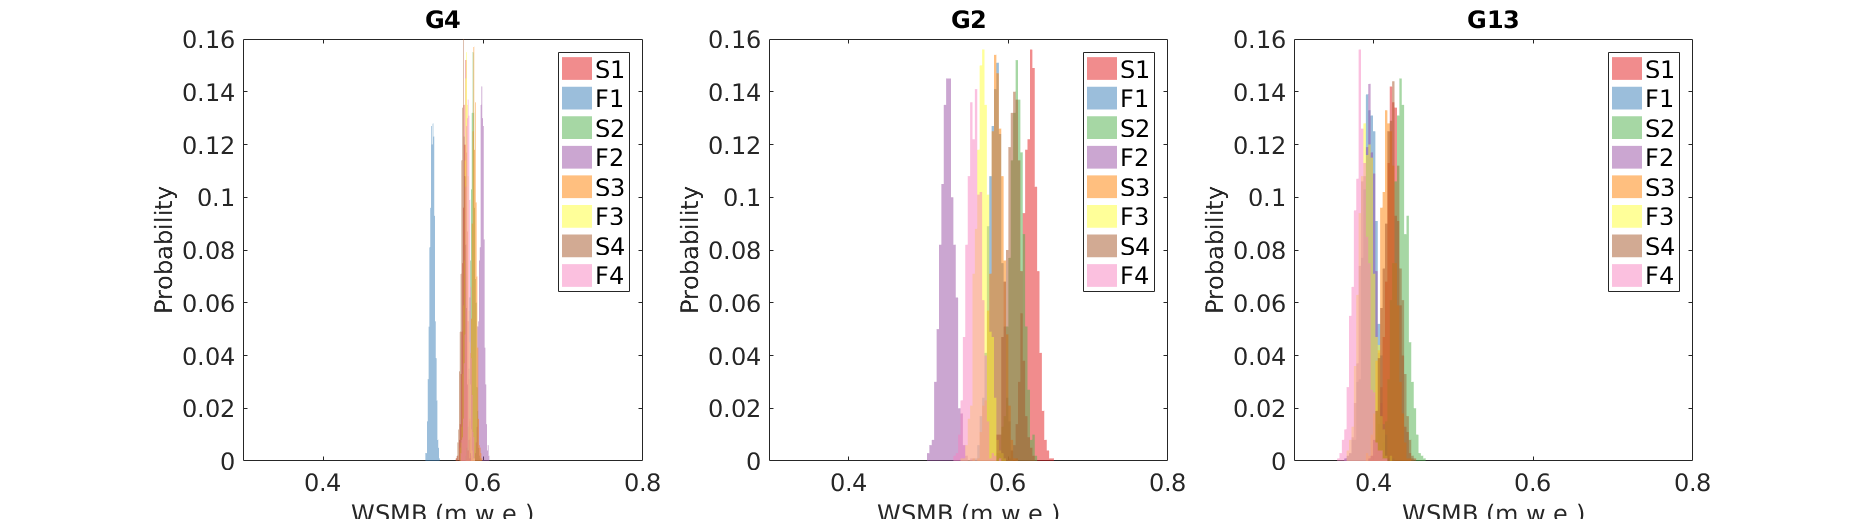
\includegraphics[width=1.2\textwidth]{WSMB_allDensityzz.png}}\\%
	\makebox[\textwidth][c]{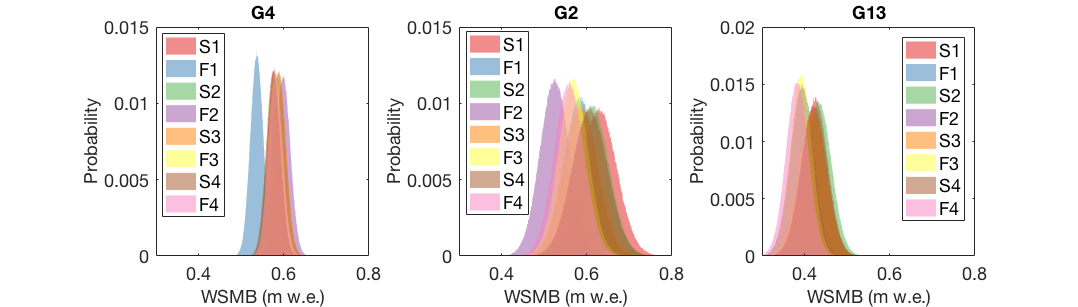
\includegraphics[width=1.2\textwidth]{WSMB_allDensityBeta.png}}\\%
	\makebox[\textwidth][c]{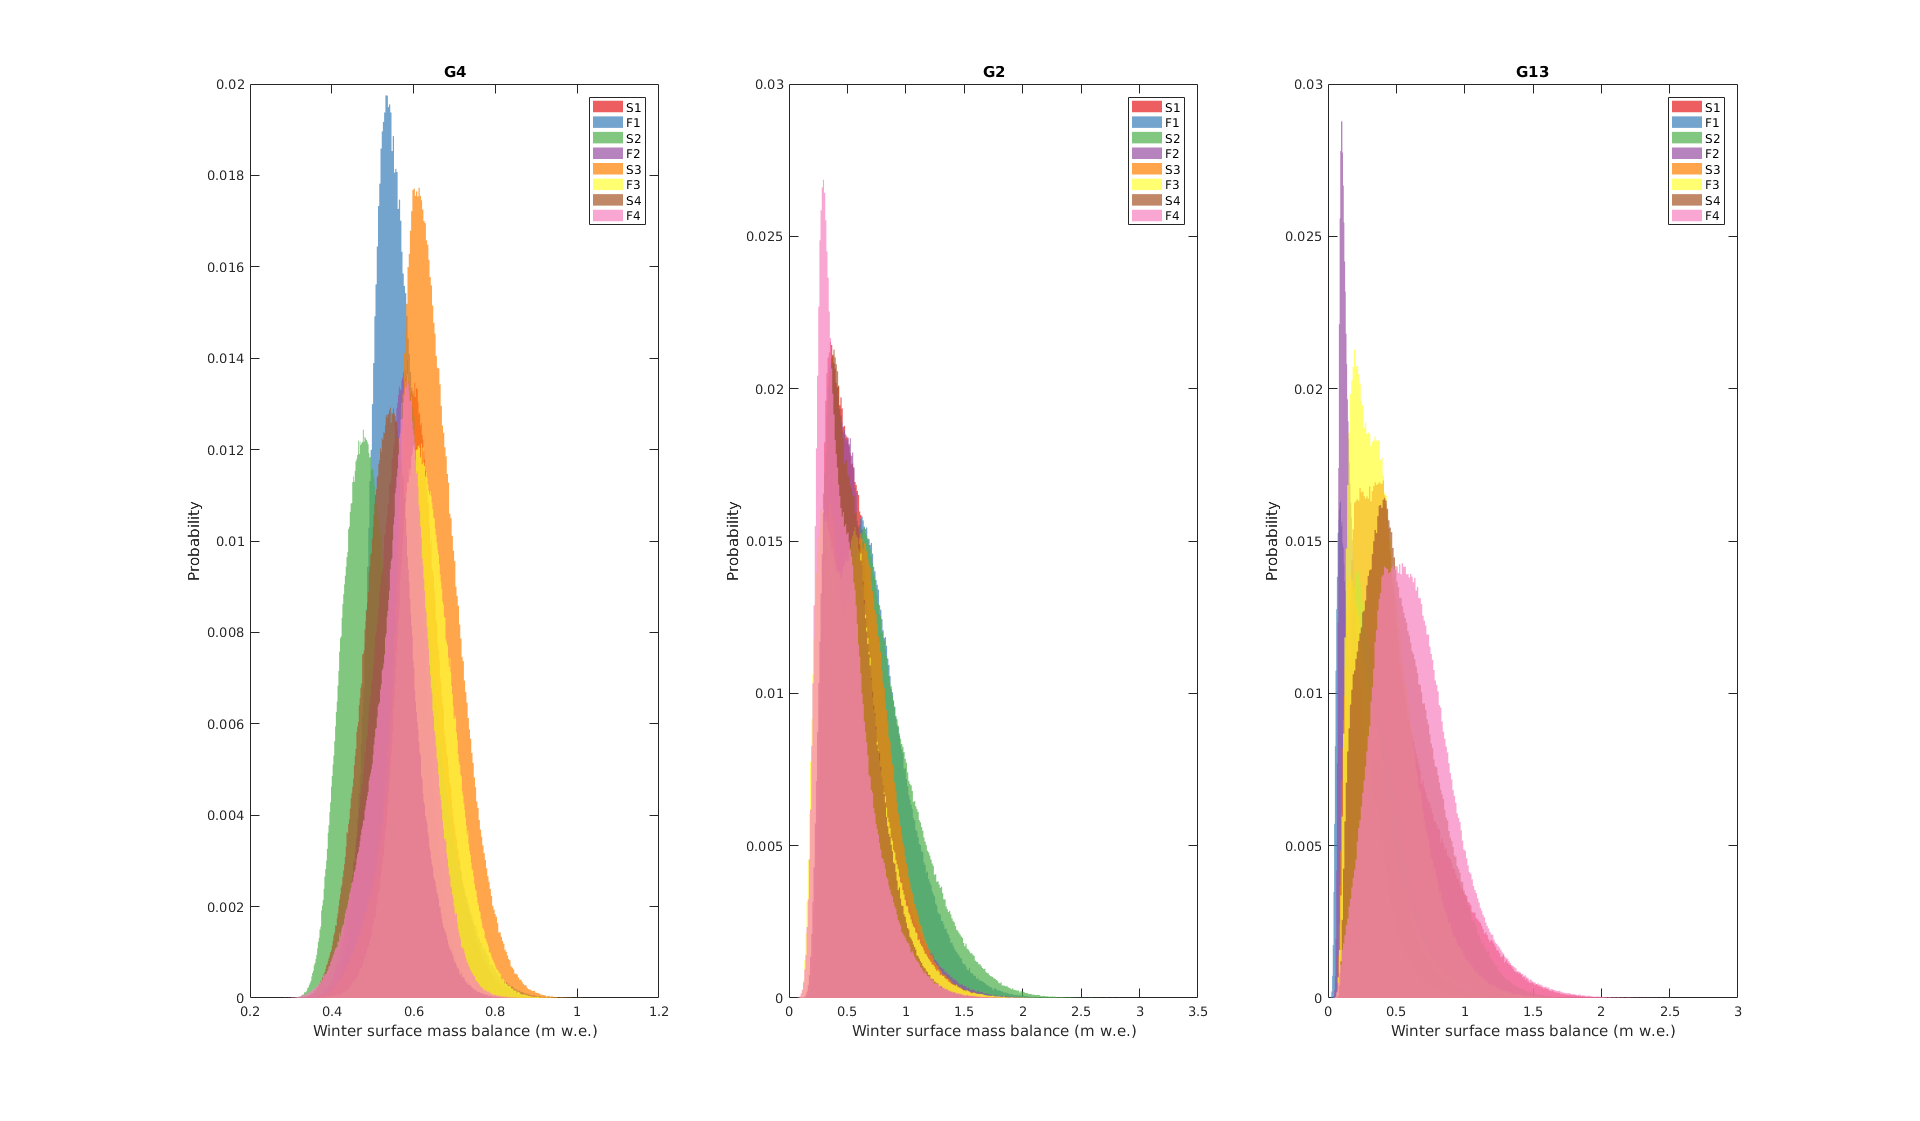
\includegraphics[width=1.2\textwidth]{WSMB_allDensityBetaNzz.png}}%
	\caption{Distribution of winter surface mass balance (WSMB). (Top) WSMB values obtained from a Monte Carlo sampling of normally distributed SWE variation (obtained from zigzag measurements) about the local SWE value. (Middle) WSMB values obtained from a Monte Carlo sampling of normally distributed regression coefficients. (Bottom) WSMB values obtained using both SWE variability and regression coefficient variability. Eight different density interpolation methods are used to obtain SWE values used in the regression.}
	\label{fig:WSMB_allDensity}
\end{figure}


\begin{figure}[H]
	\centering
	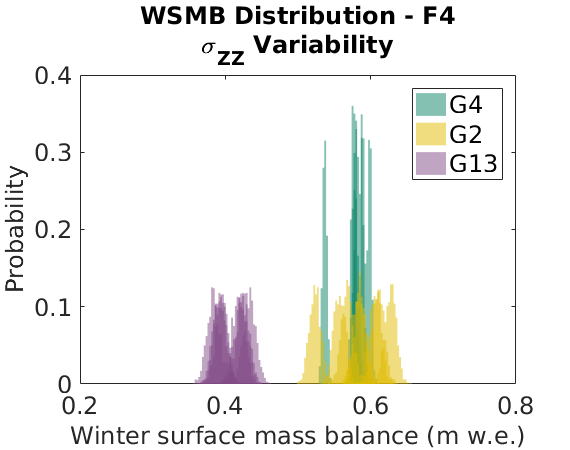
\includegraphics[width =0.5\textwidth]{WSMB_zz.png}\\
	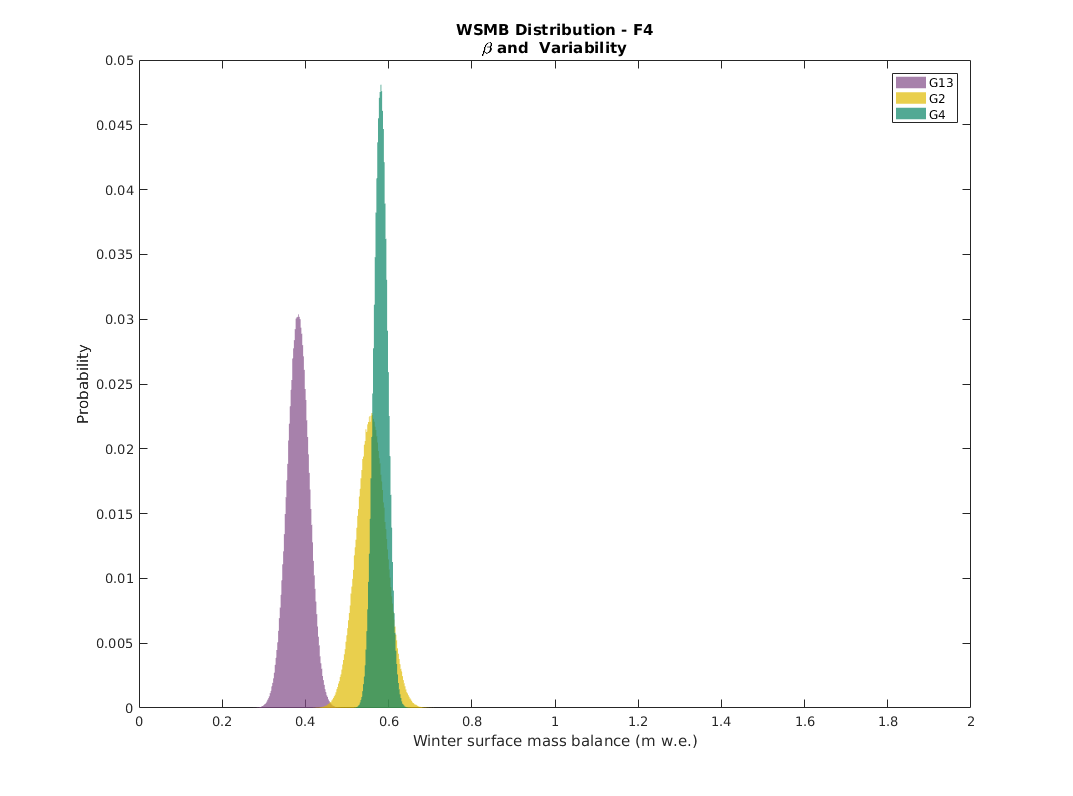
\includegraphics[width =0.5\textwidth]{WSMB_beta.png}\\
	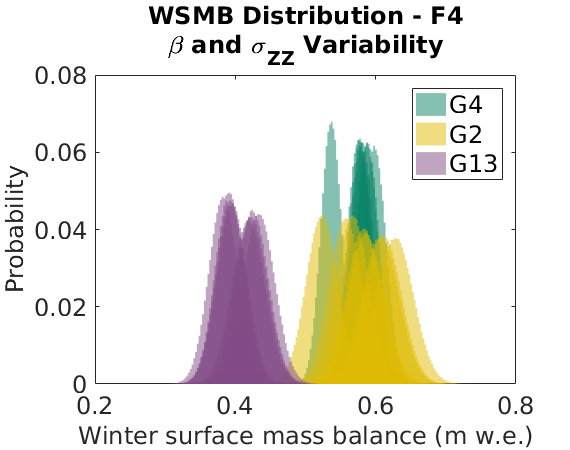
\includegraphics[width =0.5\textwidth]{WSMB_betaNzz.png}\\
	\caption{Distribution of winter surface mass balance (WSMB). (a)  WSMB values obtained from a Monte Carlo sampling of normally distributed regression coefficients. (b) WSMB values obtained as in (a) but with the addition of a Monte Carlo sampling of normally distributed SWE variation (obtained from zigzag measurements) about the local SWE value. Only data for density interpolation option F4 are shown.}
	\label{fig:WSMB_oneDensity}
\end{figure}

\begin{figure}[H]
	\centering
	\makebox[\textwidth][c]{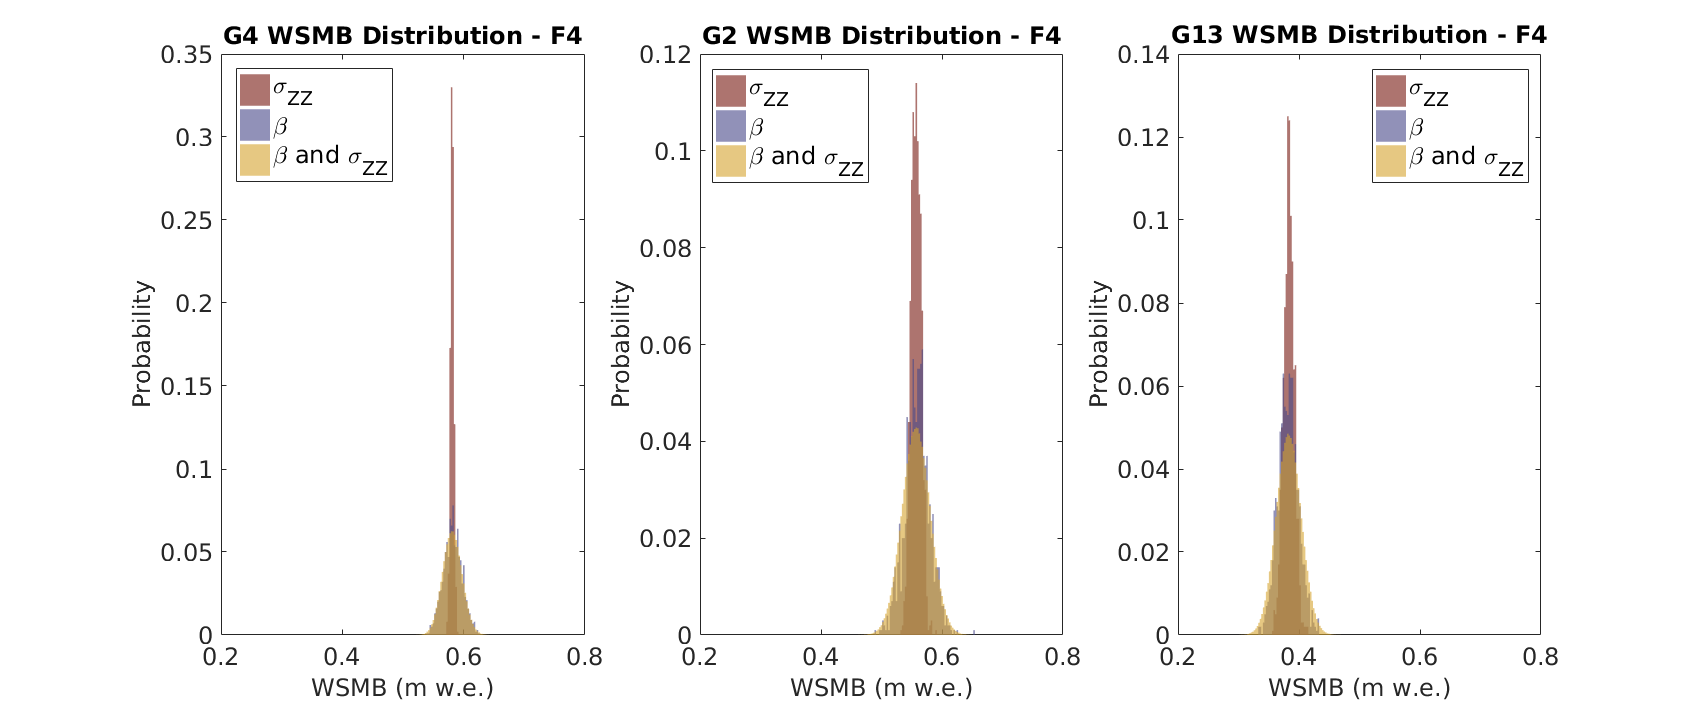
\includegraphics[width =1.2\textwidth]{WSMB_compareBetaAndZZBeta.png}}\\
	\caption{Comparison of winter surface mass balance distribution when variation due to SWE measurement ( $\sigma_{ZZ}$) and variation due to regression coefficient estimation is included ($\beta$) as well as when variation from both regression coefficient estimation and observed SWE variation within a grid cell is included ($\beta$ and $\sigma_{ZZ}$). }
	\label{fig:WSMB_compareBetaAndZZBeta}
\end{figure}

\begin{figure}[H]
	\centering
	\makebox[\textwidth][c]{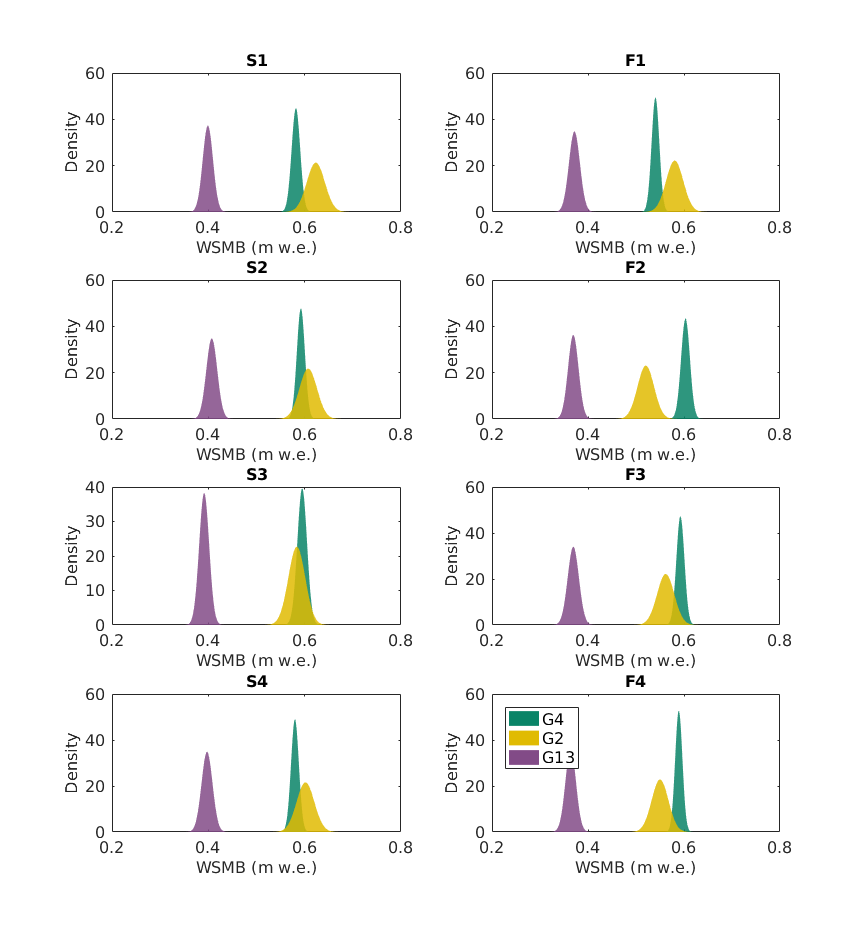
\includegraphics[width =1.2\textwidth]{WSMB_Distributionzz.png}}\\
	\caption{Winter surface mass balance distribution for eight density interpolation options when variation due to SWE measurement ( $\sigma_{ZZ}$) is included. }
	\label{fig:WSMB_Distributionzz}
\end{figure}
\begin{figure}[H]
	\centering
	\makebox[\textwidth][c]{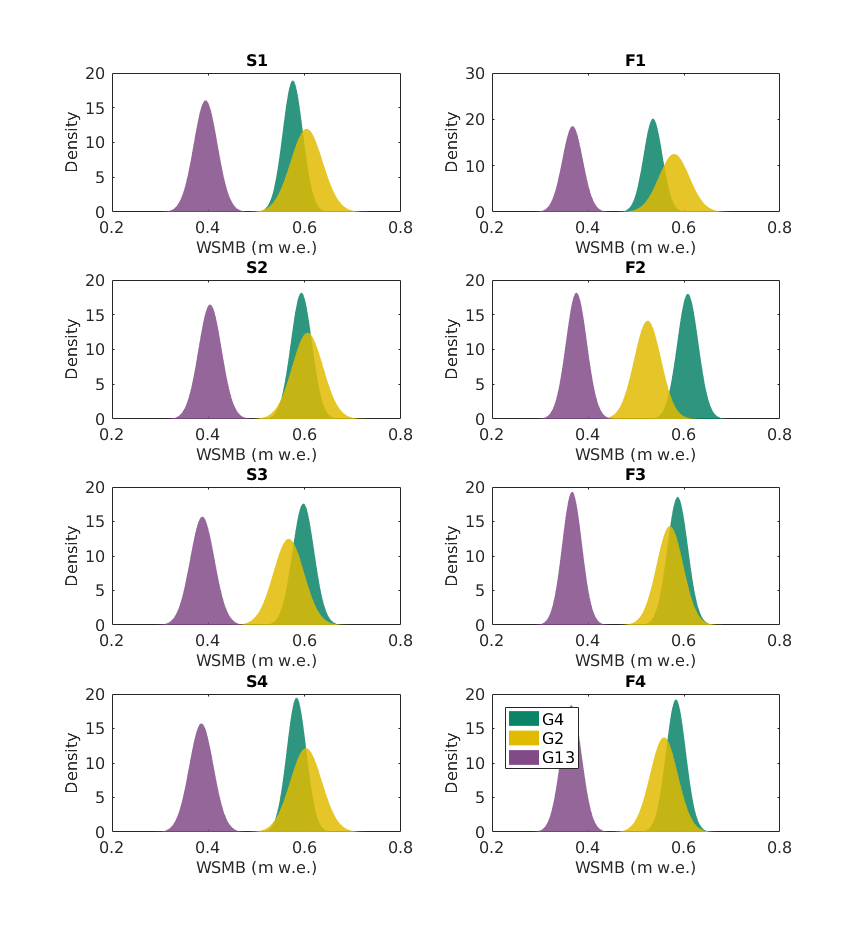
\includegraphics[width =1.2\textwidth]{WSMB_Distributionbeta.png}}\\
	\caption{Winter surface mass balance distribution for eight density interpolation options when variation due to regression coefficient estimation ( $\beta$) is included. }
	\label{fig:WSMB_Distributionbeta}
\end{figure}
\begin{figure}[H]
	\centering
	\makebox[\textwidth][c]{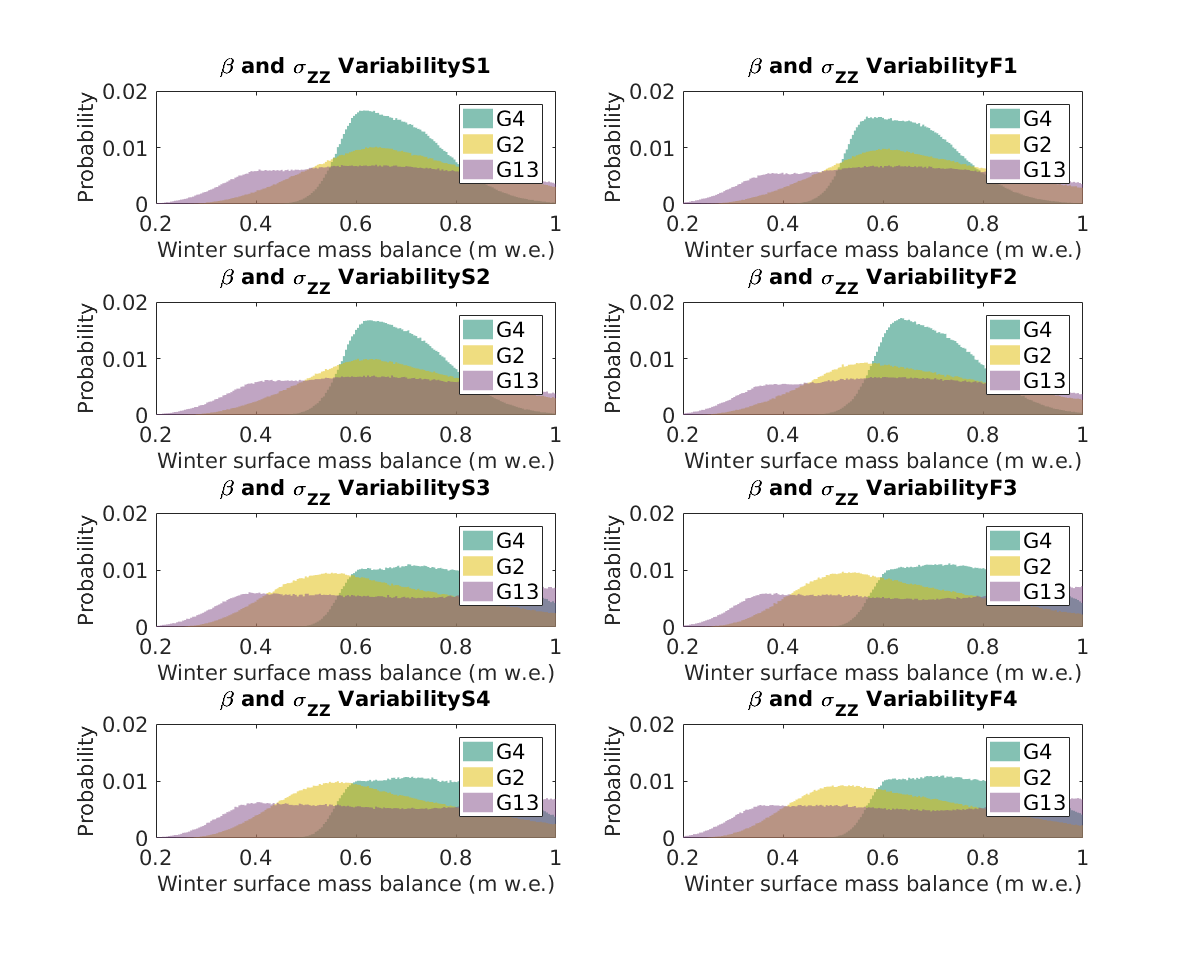
\includegraphics[width =1.2\textwidth]{WSMB_DistributionbetaNzz.png}}\\
	\caption{Winter surface mass balance distribution for eight density interpolation options when variation due to regression coefficient estimation and SWE measurement ($\beta$ and $\sigma_{ZZ}$) is included. }
	\label{fig:WSMB_DistributionbetaNzz}
\end{figure}

\begin{figure}[H]
	\centering
	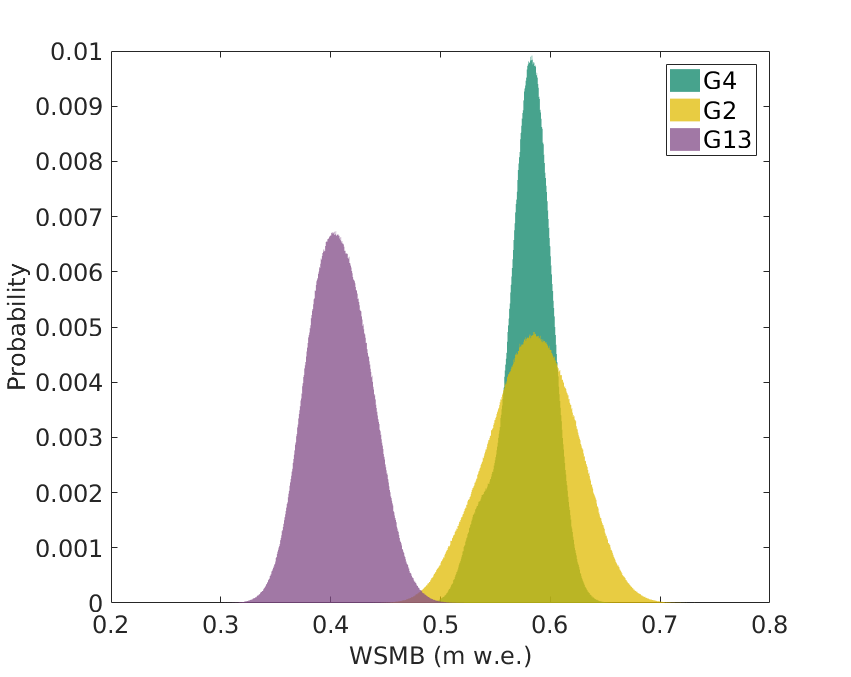
\includegraphics[width =\textwidth]{WSMB_dNbetaNzz.png}
	\caption{Total winter surface mass balance (WSMB) distribution. Variability from density interpolation options, regression coefficient estimation and SWE measurement is included. }
	\label{fig:WSMB_dNbetaNzz}
\end{figure}

%%%%%%%%%%%%%%%%%%%%%
\bibliography{/home/glaciology1/Documents/MastersDocuments/MastersLit}
\bibliographystyle{igs}
%%%%%%%%%%%%%%%%%%%%%

\end{document} 